%------------------------------------------------
%	PACKAGES AND DOCUMENT CONFIGURATIONS
%------------------------------------------------
\documentclass[11pt]{article}
\usepackage{amsmath} % Required for some math elements
\usepackage{hyperref} 
\usepackage{xcolor}
\usepackage{lipsum} 
\usepackage{cite}
\usepackage{graphicx} % Required for the inclusion of images
\usepackage{algorithmic}
\usepackage{array}
\usepackage{bookmark}
\usepackage{listings}
\usepackage{amssymb}
\usepackage{enumitem}
\usepackage{pythonhighlight}
\usepackage[T1]{fontenc}
\usepackage{inconsolata}
\usepackage[margin=16mm]{geometry}
\usepackage[caption=false, font=footnotesize]{subfig}
\usepackage[active,tightpage]{preview}

\renewcommand{\PreviewBorder}{1in}
\newcommand{\Newpage}{\end{preview}\begin{preview}}

\newlist{steps}{enumerate}{1}
\setlist[steps, 1]{label = Step \arabic*:}

\hypersetup{ %color attributes of citation, link, etc.
    colorlinks=true,
    linkcolor=blue,
    filecolor=gray,      
    urlcolor=blue,
    citecolor=blue,
}

\newcommand{\matlab}{\textsc{Matlab }} %very important and totally necessary addition

\newcommand\Item[1][]{%
  \ifx\relax#1\relax  \item \else \item[#1] \fi
  \abovedisplayskip=0pt\abovedisplayshortskip=0pt~\vspace*{-\baselineskip}}

%----------------------------------
%	DOCUMENT INFORMATION
%----------------------------------
 
\title{ECEN321 : Noise \\ Lab 2 Submission}
\author{Daniel Eisen : 300447549}
\date{\today}

\begin{document}
\begin{preview}
\maketitle
%-----------------------------
%	DOCUMENT CONTENT
%-----------------------------
\section{Introduction}
Noise, when pertaining to taking measurements, represents an uncertainty of the true value of the measured parameter. When these values are further used, i.e functions are applied to said measurements this error propagates. Hence the necessity in characterising and possibly mitigating the noise and/or its effect. This lab investigates various angles of error propagation and mitigation.

\section{Theory}
\begin{enumerate}
        \item Amplification of the (noisy) DC signal represents a linear function of that measurement. Thus the mean and uncertainty of the that functions result can be estimated. 
        $$U = aX+b = 10X+0$$ 
        $$\mathrm{mean:\;}\mu_U=a\mu_X+b = 10 \cdot 3 = 30$$
        $$\sigma_U=|a|\sigma_X = |10| \cdot 2 = 20$$
        \item To increase precision, multiple measurements can be taken and averaged. The basis of why this works is that the mean for repeated (assumed identical) measurements remains the same where the variance decreases by a factor of $\frac{1}{N}$:
        $$\mu_{\frac{1}{N}(X_{1}+{\dots}+X_{N})}=\frac{1}{N}E\{X_{1}+{\dots}+X_{N}\}=\frac{1}{N}(\mu_{X}+{\dots}+\mu_{X}) = \frac{N}{N}\mu_X = \mu_X$$
        $$\sigma_{\frac{1}{N}(X_{1}+{\dots}+X_{N})} = \frac{1}{N^2}N\sigma^2_X=\frac{1}{N}\sigma^2_X$$
        Therefore, for 16 repeated measurements, the various with decrease by 1/16, or the std by 1/4. i.e $\sigma=2 \rightarrow \sigma=0.5$
        \item Covariance is a measure of how two variables change together, but its magnitude is unbounded, so it is difficult to interpret. 
        $$Cov(X,Y) = \mu_{XY} - \mu_{X}\mu_{Y}$$
        By dividing covariance by the product of the two standard deviations, one can calculate the normalized version of the statistic. This is the correlation coefficient.
        $$\rho_{XY} = \frac{Cov(X,Y)}{\sigma_{X}\sigma_{Y}}$$
        The correlation coefficient is a statistical measure of the strength of the relationship between the relative movements of two variables, range[-1.0 1.0].
        \item For the linear combination of two variable,eg in the case $X \pm Y$, the combination of their errors can be written as:
        $$\sigma_{X+Y} = \sqrt{\sigma^2_X + \sigma^2_Y}$$
        Note: The convolution method states that for 2+ errors, the distribution for the combined error can be obtained via convolution.
\end{enumerate}

\Newpage
\section{Results}
\begin{enumerate}
        \item Amplified Noise \\
        \inputpython{../py/lab2.py}{7}{16}
        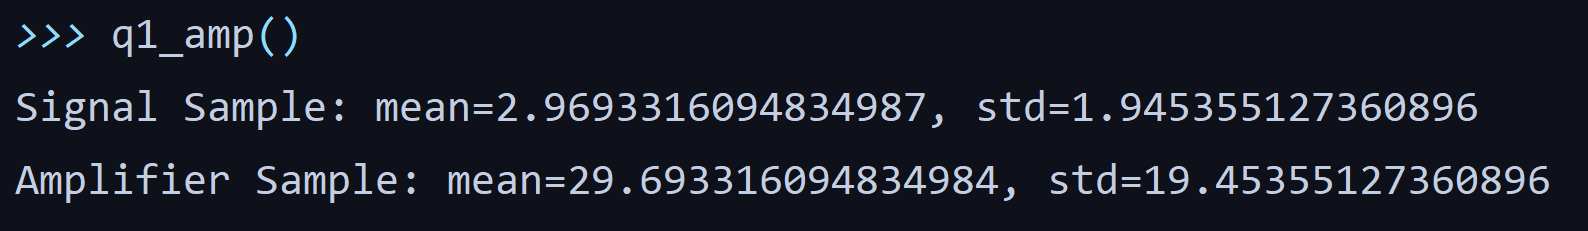
\includegraphics[width=\linewidth]{inc/q1_out.png} \\
        Result of the included python codes amplifier simulation. These can be seen to confirm the estimated mean and std in section 2.1, with noise being subject to the same scaling (of the function) as the "true" value.


        \item Averaged Measurements \\
        \inputpython{../py/lab2.py}{20}{29}
        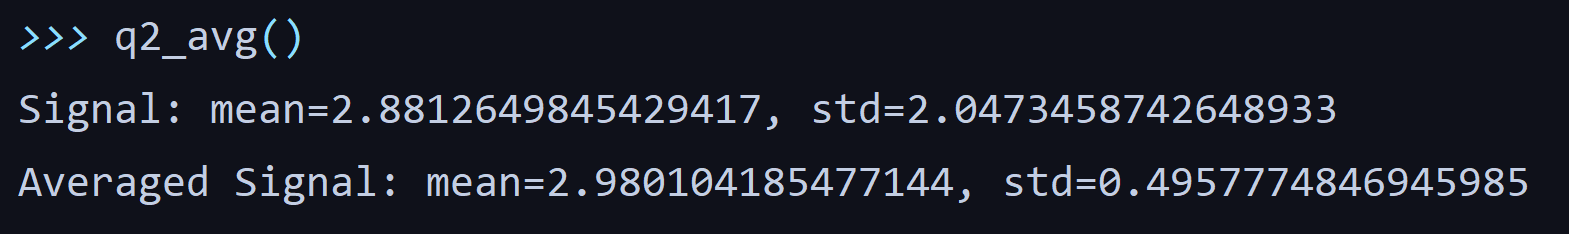
\includegraphics[width=\linewidth]{inc/q2_out.png} \\
        Results of script confirm section 2.2. Showing preserved mean with a std reduction of 1/4, ~2 to ~0.5. The results of the average would be (as shown in section 2) improved by a greater N of trials. 

        \item Covariance and Correlation \\
        \inputpython{../py/lab2.py}{33}{47}
        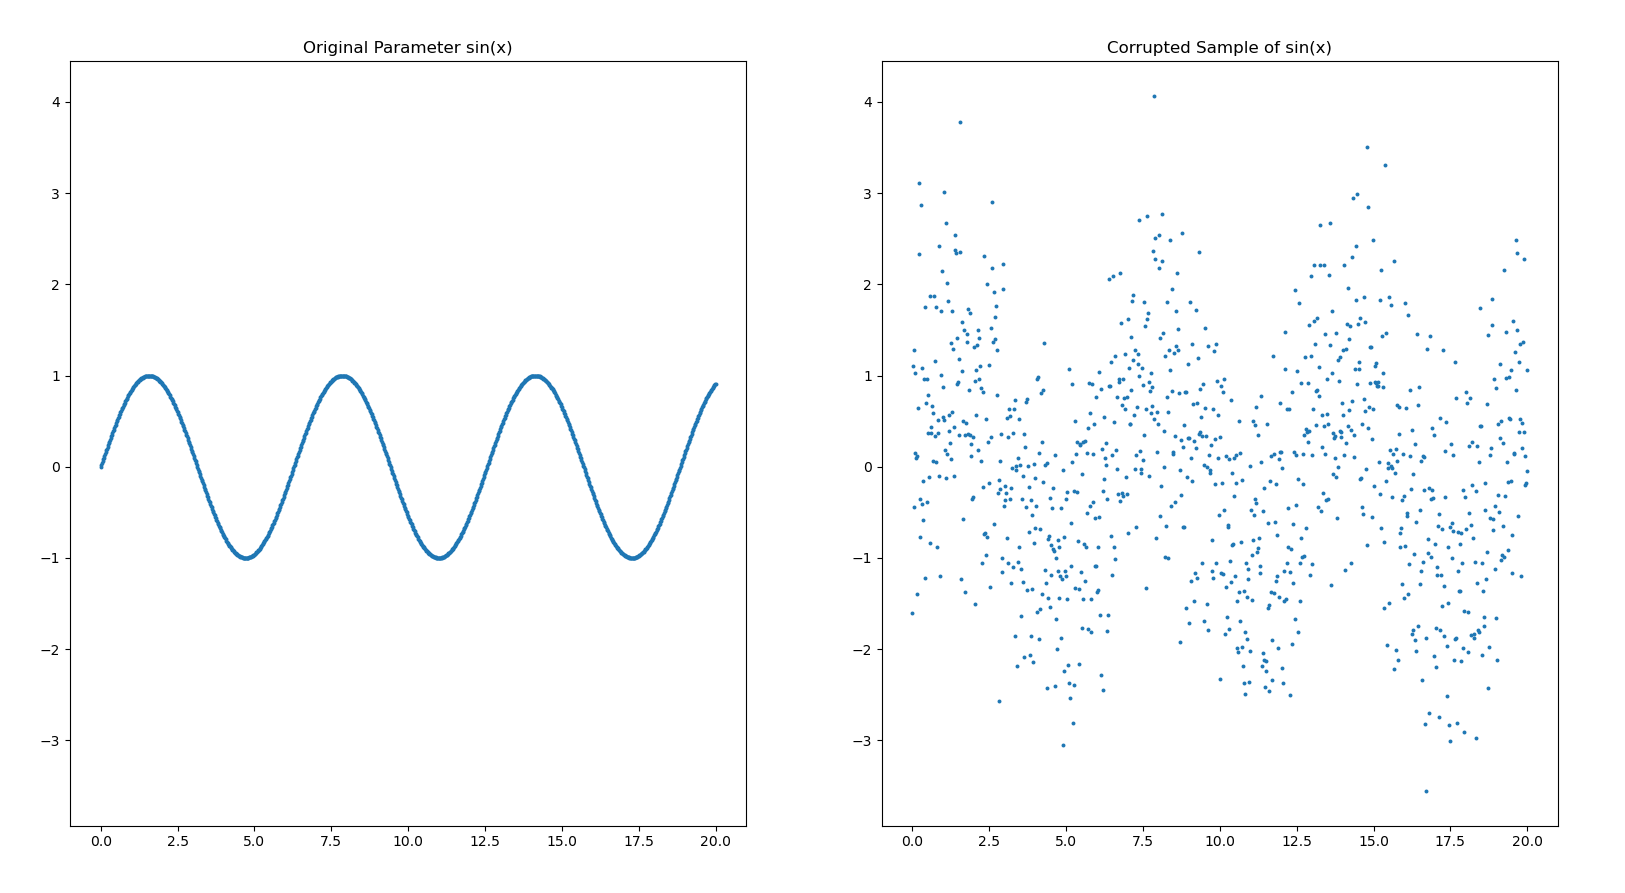
\includegraphics[width=\linewidth]{inc/q3_plot.png} \\
        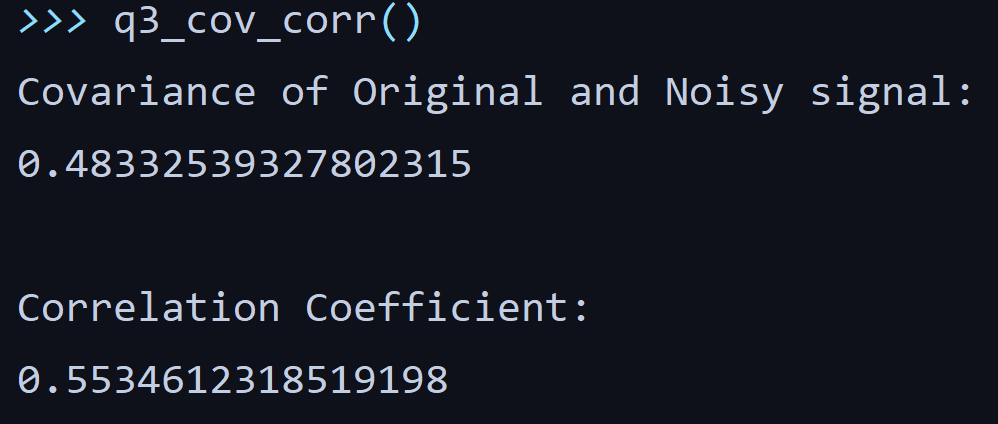
\includegraphics[width=\linewidth]{inc/q3_out.png} \\ \\
        Corrupting the original signal with noise to this degree can be see to visually distort the signal to quite a large degree. This breakdown in the samples relationship to its original signal is confirmed be the given calculation of the the correlation coefficient.

        \item Combined Uncertainty \\
        \inputpython{../py/lab2.py}{51}{73}
        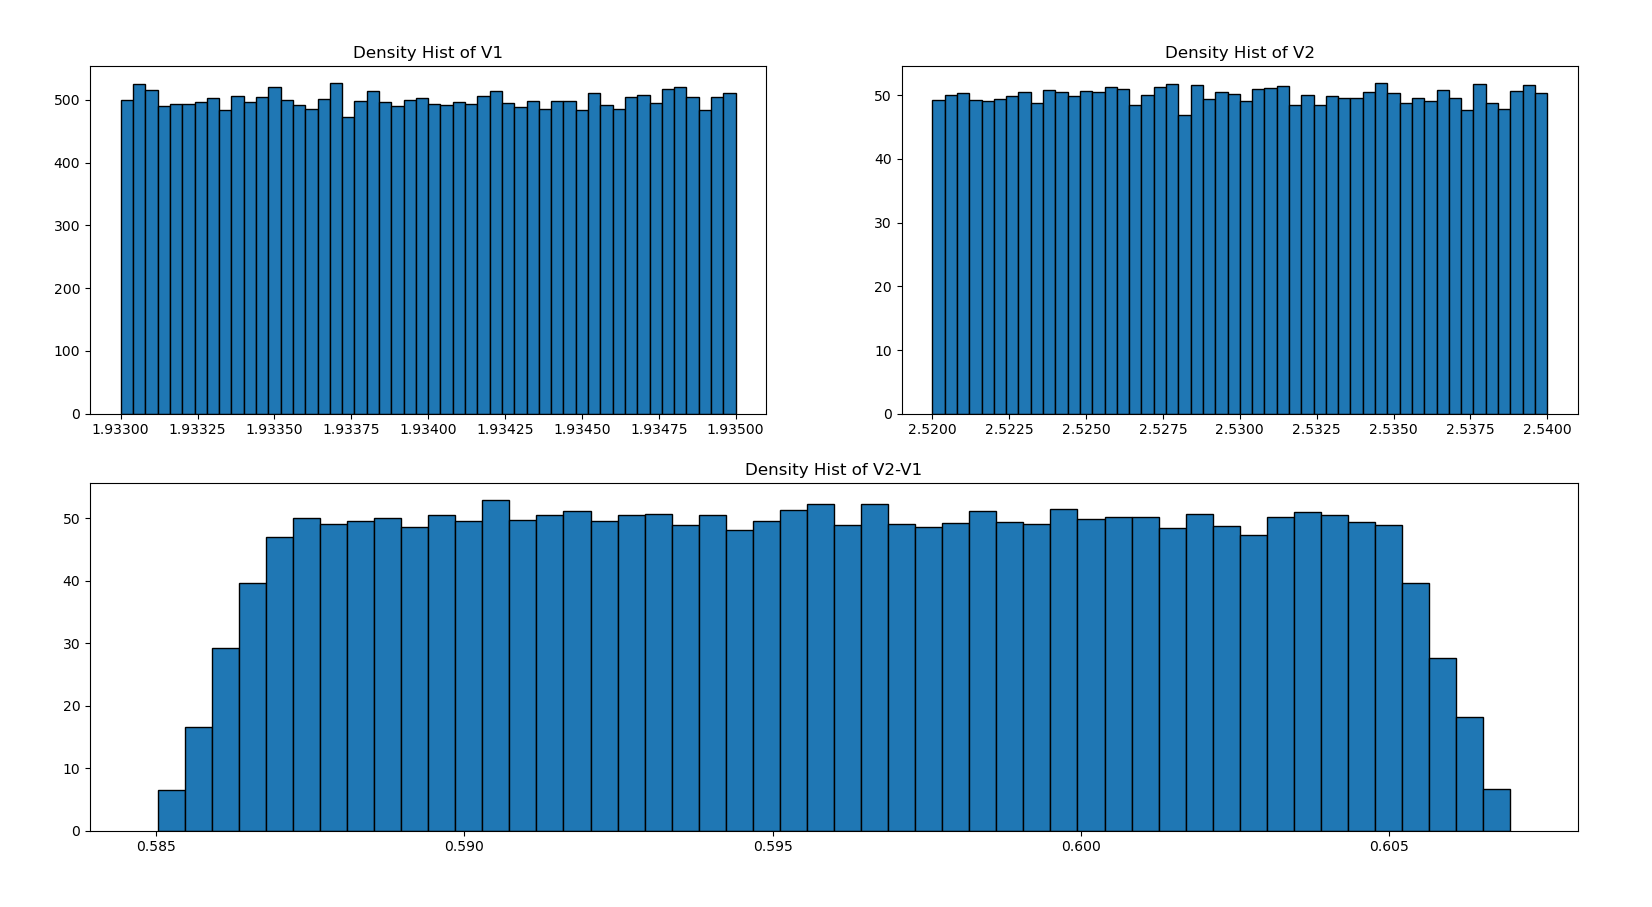
\includegraphics[width=\linewidth]{inc/q4_plot.png} \\
        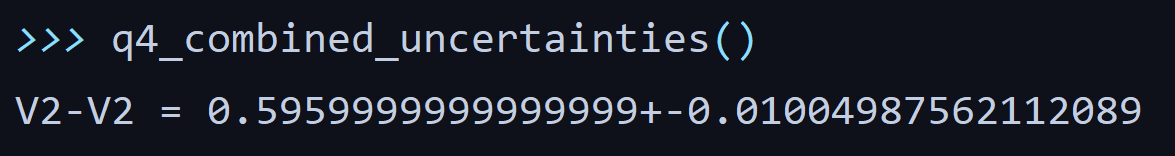
\includegraphics[width=\linewidth]{inc/q4_out.png} \\ \\ \\
        Numpy's histogram function was used to produce the above density plots of the V1, V2 and V2-V1. The plotted estimate of V2-V1's pdf corroborates with the outputs calculation of $0.596\pm0.01$. It shape is also consistent with the convolution method referenced in section 2.4, \tiny{i.e the convolution of 2 square pulses resulting in a trapezium.}
\end{enumerate}

\Newpage
\section*{Appendix}
\subsection*{Full Python Script}
\inputpython{../py/lab2.py}{1}{100}

\end{preview}
\end{document}